% ============================================================================
%  C3 System Database Management -- Deliverable #2 component design
%  Owner: Renuka Prasad Patwari
% ============================================================================
\section{Component Overview}

\subsection{Purpose}
C3 System Database Management is the data and intelligence core of HomeAI Cloud. It carries four
responsibilities. It runs the AI inference sub-service that turns each uploaded clip into a ranked set of
home sound labels using the pre-trained YAMNet model. It maintains the versioned data dictionary for the whole
platform schema. It provides paginated, permission-scoped record browsing over every entity, plus cross-store
integrity validation and a demo-data seed and backup job. It computes each house's hourly activity pattern and
an anomaly score against the learned baseline.

C3 owns steps 3 and 4 of the clip-to-alert flow. It picks up a clip that C1 has left in \texttt{media\_events}
with status \texttt{queued}, classifies it, stores the detection, sets the clip to \texttt{analyzed}, and hands off
to C2 by calling \texttt{POST /alerts/evaluate}. Classification is audio only: a video clip is classified on its
audio track; there is no visual model.

\subsection{Objectives}
\begin{enumerate}
\item Classify every uploaded clip and persist a ranked, auditable detection with its model version.
\item Resolve the 521 YAMNet classes to seven home labels with per-label thresholds and a frame-combine rule (the label map, Section~\ref{sec:c3-tbd1}).
\item Keep the pipeline idempotent and crash-safe: each clip is claimed by one worker, retried at most three times, and never lost.
\item Give staff one safe, scoped, paginated way to read any platform record, and publish a versioned data dictionary.
\item Detect cross-store integrity faults (orphans, stuck clips, failed handoffs) before they reach a dashboard.
\item Roll detections up into hourly activity patterns per room with an anomaly score.
\end{enumerate}

\subsection{Function scope}
\begin{longtable}{L{6.4cm}L{8.4cm}}
\caption{C3 function scope}\label{tab:c3-scope}\\
\toprule
\textbf{In C3} & \textbf{Out of C3 (owner)} \\
\midrule
\endfirsthead
\caption[]{C3 function scope (continued)}\\
\toprule
\textbf{In C3} & \textbf{Out of C3 (owner)} \\
\midrule
\endhead
AI inference sub-service (worker, YAMNet runner, label mapper) & Clip upload and \texttt{media\_events} creation (C1) \\
\texttt{ml\_models}, \texttt{integrity\_reports}, \texttt{data\_dictionary\_versions} (PostgreSQL) & Alert rules, evaluation and the alert status machine (C2) \\
\texttt{ai\_detections}, \texttt{activity\_patterns} (MongoDB) & Authentication, token issue, dashboards (C4) \\
Data dictionary, record browsing, integrity validation, seed and backup & Writes to any other component's data (C3 reads them read-only) \\
\bottomrule
\end{longtable}
\textbf{Assumption.} C3 writes only the processing fields of C1's \texttt{media\_events}
(\texttt{status}, \texttt{attempts}, \texttt{claimed\_at}, \texttt{error}, \texttt{detection\_id}, \texttt{handoff\_status}).

\subsection{Usage}
\begin{longtable}{L{3.0cm}L{4.0cm}L{7.8cm}}
\caption{C3 actors}\label{tab:c3-actors}\\
\toprule
\textbf{Actor} & \textbf{Interface} & \textbf{Typical use} \\
\midrule
\endfirsthead
\caption[]{C3 actors (continued)}\\
\toprule
\textbf{Actor} & \textbf{Interface} & \textbf{Typical use} \\
\midrule
\endhead
Inference worker (system) & MongoDB claim loop & Classifies every queued clip, no login \\
\texttt{cloud\_staff} & Database Records page $\rightarrow$ C3 REST & Browse records, run integrity checks, export the dictionary, re-classify or requeue clips \\
\texttt{iot\_staff}, \texttt{house\_owner} & C3 REST through C4 pages & Scoped reads of their own detections and activity patterns \\
C4 dashboard (service) & \texttt{GET /records}, service JWT & Detection counts for statistics \\
Operator & Deployment tooling & Seed demo data, run and verify backups \\
\bottomrule
\end{longtable}

\subsection{Function partition}
\figH{C3/c3-partition-overview}{0.66}{C3 function partition: five sub-functions under System Database Management}{fig:c3-partition}

\begin{longtable}{L{2.2cm}L{8.4cm}L{4.0cm}}
\caption{C3 functional requirements mapped to sub-functions}\label{tab:c3-fr}\\
\toprule
\textbf{Req} & \textbf{Requirement (abridged)} & \textbf{Sub-function} \\
\midrule
\endfirsthead
\caption[]{C3 functional requirements mapped to sub-functions (continued)}\\
\toprule
\textbf{Req} & \textbf{Requirement (abridged)} & \textbf{Sub-function} \\
\midrule
\endhead
FR-C3-01 & Classify a clip with the pre-trained model; persist ranked labels, confidence and model version & AI inference sub-service \\
FR-C3-02 & Maintain a versioned data dictionary of every table, collection, field and owner & Data dictionary \\
FR-C3-03 & Paginated, permission-scoped record browsing across houses, feeds, clips, detections and alerts & Record browsing and query \\
FR-C3-04 & Integrity validation that reports orphan references between the relational and document stores & Integrity validation \\
FR-C3-05 & Idempotent demo-data seed and a database backup job & Seed and backup \\
FR-C3-06 & Hourly activity profile per room and day with an anomaly score & AI inference sub-service (activity rollup) \\
\bottomrule
\end{longtable}

\subsection{Component function specification}
\begin{longtable}{L{1.1cm}L{2.6cm}L{3.0cm}L{3.2cm}L{4.8cm}}
\caption{C3 function specification}\label{tab:c3-funcspec}\\
\toprule
\textbf{ID} & \textbf{Function} & \textbf{Input / trigger} & \textbf{Output} & \textbf{Pre- / post-conditions} \\
\midrule
\endfirsthead
\caption[]{C3 function specification (continued)}\\
\toprule
\textbf{ID} & \textbf{Function} & \textbf{Input / trigger} & \textbf{Output} & \textbf{Pre- / post-conditions} \\
\midrule
\endhead
F-01 & Claim clip & poll every 2 s & MediaEvent \texttt{processing} & Atomic; only one worker gets a clip \\
F-02 & Classify clip & claimed clip & Detection & Post: ranked labels, \texttt{top\_label}, model version stored \\
F-03 & Hand off to C2 & detection & C2 decision & Post: \texttt{handoff\_status} \texttt{done} or \texttt{pending} \\
F-04 & Re-classify on demand & \texttt{media\_id}, \texttt{force} & Detection & Pre: \texttt{cloud\_staff}; 409 if already analysed and not forced \\
F-05 & Browse records & entity, filters, page & Page of rows & Post: tenant/house scope always applied \\
F-06 & Data dictionary & entity?, version? & Dictionary document & Post: read-only; versions immutable \\
F-07 & Integrity check & scope & Report id (202), findings & Async; one running check per tenant \\
F-08 & Requeue clip & \texttt{media\_id} & MediaEvent \texttt{queued} & Pre: status \texttt{failed}; attempts reset \\
F-09 & Activity pattern & house, room, date & hours[24], anomaly score & Post: updated per detection \\
F-10 & Seed / backup & operator job & seed data; snapshot & Seed idempotent; daily backups kept 14 days \\
\bottomrule
\end{longtable}

% ============================================================================
\section{Component Application Interface Design and Analysis}

\subsection{API conventions}
Paths are relative to \texttt{https://<host>/api/v1}; JSON over HTTPS with a C4-issued bearer JWT. Success bodies
are \texttt{\{"data": ..., "meta": \{"page", "page\_size", "total"\}\}} and errors \texttt{\{"error": \{"code", "message", "details"\}\}}.
Keys are UUID strings in every store, so the same identifier joins PostgreSQL and MongoDB (\texttt{media\_id},
\texttt{detection\_id}). Long-running work returns \texttt{202 Accepted} with a resource id. The OpenAPI contract is frozen at Deliverable~\#2.

\subsection{API catalogue}
\begin{longtable}{L{1.2cm}L{4.8cm}L{3.0cm}L{1.2cm}L{4.4cm}}
\caption{C3 API catalogue}\label{tab:c3-catalogue}\\
\toprule
\textbf{Method} & \textbf{Path} & \textbf{Access} & \textbf{OK} & \textbf{Purpose} \\
\midrule
\endfirsthead
\caption[]{C3 API catalogue (continued)}\\
\toprule
\textbf{Method} & \textbf{Path} & \textbf{Access} & \textbf{OK} & \textbf{Purpose} \\
\midrule
\endhead
POST & \texttt{/inference/classify} & cloud\_staff & 200 & Re-run classification of one clip \\
POST & \texttt{/media-events/\{media\_id\}/requeue} & cloud\_staff & 200 & Put a \texttt{failed} clip back in the queue \\
GET & \texttt{/models/active} & staff & 200 & Active model and label map version \\
GET & \texttt{/records/\{entity\}} & role-scoped & 200 & Browse an entity (Table~\ref{tab:c3-scope-dt}) \\
GET & \texttt{/records/\{entity\}/\{id\}} & role-scoped & 200 & One record \\
GET & \texttt{/data-dictionary} & cloud\_staff & 200 & Current dictionary (optional \texttt{entity}, \texttt{version}) \\
GET & \texttt{/data-dictionary/versions} & cloud\_staff & 200 & Dictionary version list \\
POST & \texttt{/integrity-checks} & cloud\_staff & 202 & Start a check, returns \texttt{report\_id} \\
GET & \texttt{/integrity-reports/\{report\_id\}} & cloud\_staff & 200 & Status and findings \\
GET & \texttt{/activity-patterns} & owner, staff & 200 & \texttt{house\_id}, \texttt{room\_id?}, \texttt{date} \\
\bottomrule
\end{longtable}

\subsection{Web service API: POST /inference/classify}
Re-runs classification of one clip synchronously and persists the detection. The normal path is the worker
(Section~\ref{sec:c3-seq}); both use the same \texttt{ClassificationPipeline} and both hand off to C2.
\begin{longtable}{L{2.6cm}L{1.4cm}L{1.8cm}L{1.1cm}L{7.0cm}}
\caption{POST /inference/classify body}\\
\toprule
\textbf{Parameter} & \textbf{In} & \textbf{Type} & \textbf{Req.} & \textbf{Description} \\
\midrule
\endfirsthead
\caption[]{POST /inference/classify body (continued)}\\
\toprule
\textbf{Parameter} & \textbf{In} & \textbf{Type} & \textbf{Req.} & \textbf{Description} \\
\midrule
\endhead
\texttt{media\_id} & body & uuid & yes & Clip in \texttt{media\_events}, in the caller's scope \\
\texttt{force} & body & bool & no & Replace an existing detection (default false) \\
\bottomrule
\end{longtable}
\begin{Shaded}
\begin{Code}
POST /api/v1/inference/classify { "media_id": "9b1e2f40-...", "force": true }
200 OK { "data": { "detection_id": "3f2a7c10-...", "media_id": "9b1e2f40-...", "house_id": "a3d9f7e2-...",
                   "top_label": "glass_break", "top_confidence": 0.78,
                   "labels": [ {"label":"glass_break","confidence":0.78}, {"label":"speech","confidence":0.33} ],
                   "model": {"name":"yamnet","version":"1.0.0"}, "alert_decision": "alert" } }
\end{Code}
\end{Shaded}
\noindent Errors: \texttt{404 not\_found}, \texttt{409 already\_analyzed} (and \texttt{force} false), \texttt{422 unreadable\_clip},
\texttt{503 dependency\_unavailable}.

\subsection{Web service API: GET /records/\{entity\}}
Paginated, permission-scoped browsing. \texttt{entity} is one of \texttt{houses}, \texttt{rooms}, \texttt{feeds},
\texttt{clips}, \texttt{detections}, \texttt{alerts}, \texttt{activity\_patterns}. The scope from the token is applied
before any query runs (Table~\ref{tab:c3-scope-dt}).
\begin{longtable}{L{2.6cm}L{1.4cm}L{1.8cm}L{1.1cm}L{7.0cm}}
\caption{GET /records/\{entity\} parameters}\\
\toprule
\textbf{Parameter} & \textbf{In} & \textbf{Type} & \textbf{Req.} & \textbf{Description} \\
\midrule
\endfirsthead
\caption[]{GET /records/\{entity\} parameters (continued)}\\
\toprule
\textbf{Parameter} & \textbf{In} & \textbf{Type} & \textbf{Req.} & \textbf{Description} \\
\midrule
\endhead
\texttt{entity} & path & string & yes & Entity name (404 \texttt{unknown\_entity} otherwise) \\
\texttt{house\_id} & query & uuid & no & One house in scope (403 otherwise) \\
\texttt{from}, \texttt{to} & query & date-time & no & Window on the entity's timestamp; max 366 days \\
\texttt{filter} & query & string & no & Field equality, e.g. \texttt{top\_label:glass\_break} (whitelisted fields only) \\
\texttt{page}, \texttt{page\_size} & query & int & no & Default 1 and 25; max 100 \\
\bottomrule
\end{longtable}
\begin{Shaded}
\begin{Code}
GET /api/v1/records/detections?house_id=a3d9f7e2-...&from=2026-10-20T00:00:00Z&page=1&page_size=25
200 OK { "data": [ {"detection_id":"3f2a7c10-...","media_id":"9b1e2f40-...","top_label":"glass_break",
                    "top_confidence":0.78,"detected_at":"2026-10-24T18:40:50Z"} ],
         "meta": { "page": 1, "page_size": 25, "total": 134 } }
\end{Code}
\end{Shaded}

\subsection{Data dictionary, integrity and activity APIs}
\texttt{POST /integrity-checks} takes \texttt{\{scope: "tenant" | "house", house\_id?\}}, creates a report with status
\texttt{running} and returns \texttt{202 \{report\_id\}}; a second request while one is running returns
\texttt{409 check\_running}. \texttt{GET /integrity-reports/\{id\}} returns \texttt{status} (\texttt{running},
\texttt{done}, \texttt{failed}) and \texttt{findings[]} of \texttt{\{type, entity, id, severity\}}.
\texttt{GET /activity-patterns} returns \texttt{hours[24]}, \texttt{baseline[24]} and \texttt{anomaly\_score} for a
house, room and date. Seed and backup are operator jobs run by deployment tooling, not public endpoints.

\subsection{Outbound API: C3 $\rightarrow$ C2 POST /alerts/evaluate}
After storing a detection, C3 calls C2 with a service JWT (scope \texttt{alerts:evaluate}, issued by C4) and this body,
which matches C2's contract exactly:
\begin{Shaded}
\begin{Code}
{ "detection_id": "3f2a7c10-...", "media_id": "9b1e2f40-...", "house_id": "a3d9f7e2-...", "room_id": "c7e1b2d3-...",
  "top_label": "glass_break", "top_confidence": 0.78,
  "labels": [ {"label":"glass_break","confidence":0.78}, {"label":"speech","confidence":0.33} ],
  "detected_at": "2026-10-24T18:40:50Z" }
\end{Code}
\end{Shaded}
\noindent C2 replies \texttt{201} (alert) or \texttt{200} (no alert, or duplicate). On \texttt{5xx} or timeout C3 retries
three times (2, 4, 8 s), then marks \texttt{handoff\_status = pending}; the integrity job re-sends pending handoffs.
C2 is idempotent on \texttt{detection\_id}, so a re-send can never create a second alert.

\subsection{Error model}
\begin{longtable}{L{1.3cm}L{4.2cm}L{9.2cm}}
\caption{C3 error codes}\\
\toprule
\textbf{HTTP} & \textbf{code} & \textbf{When} \\
\midrule
\endfirsthead
\caption[]{C3 error codes (continued)}\\
\toprule
\textbf{HTTP} & \textbf{code} & \textbf{When} \\
\midrule
\endhead
401 / 403 & \texttt{unauthorized} / \texttt{forbidden} & Token invalid; entity or house outside scope \\
404 & \texttt{not\_found}, \texttt{unknown\_entity} & Unknown clip, report, version or entity \\
409 & \texttt{already\_analyzed}, \texttt{check\_running}, \texttt{not\_failed} & State rule broken \\
422 & \texttt{validation\_error}, \texttt{unreadable\_clip} & Bad filter, page or window; clip cannot be decoded \\
429 & \texttt{rate\_limited} & More than 60 record queries per minute per user \\
503 & \texttt{dependency\_unavailable} & S3, a store or C2 unreachable \\
\bottomrule
\end{longtable}

\subsection{Connectivity APIs}
\begin{longtable}{L{3.4cm}L{2.6cm}L{2.2cm}L{6.4cm}}
\caption{C3 connectivity interfaces}\label{tab:c3-conn}\\
\toprule
\textbf{Interface} & \textbf{Protocol / port} & \textbf{Auth} & \textbf{Data exchanged (sync / async)} \\
\midrule
\endfirsthead
\caption[]{C3 connectivity interfaces (continued)}\\
\toprule
\textbf{Interface} & \textbf{Protocol / port} & \textbf{Auth} & \textbf{Data exchanged (sync / async)} \\
\midrule
\endhead
Worker $\rightarrow$ MongoDB \texttt{media\_events} & TCP 27017 & Per-service user & Atomic claim \texttt{queued}$\rightarrow$\texttt{processing}; status updates (async) \\
Worker $\rightarrow$ Amazon S3 & HTTPS 443 & IAM instance role & Read clip bytes by key, read-only (sync) \\
Worker $\rightarrow$ YAMNet runner & In-process & n/a & 16 kHz mono PCM in, per-frame 521-class scores out (sync) \\
C3 $\rightarrow$ MongoDB (own) & TCP 27017 & Per-service user & Insert \texttt{ai\_detections}; upsert \texttt{activity\_patterns} \\
C3 $\rightarrow$ PostgreSQL (own) & TCP 5432 & Secrets Manager & \texttt{ml\_models} (cached 5 min), reports, dictionary versions \\
C3 $\rightarrow$ C2 \texttt{/alerts/evaluate} & HTTPS 443, internal & Service JWT & Detection handoff (async to the clip, sync call) \\
C3 $\rightarrow$ C1/C2/C4 stores & TCP, read-only users & Secrets Manager & Record browsing and integrity checks; never writes \\
C4 $\rightarrow$ C3 \texttt{/records} & HTTPS 443 & Service JWT & Detection counts for dashboards (inbound) \\
\bottomrule
\end{longtable}

\subsection{API design analysis}
\begin{longtable}{L{2.8cm}L{12.0cm}}
\caption{C3 API design decisions}\\
\toprule
\textbf{Concern} & \textbf{Decision and rationale} \\
\midrule
\endfirsthead
\caption[]{C3 API design decisions (continued)}\\
\toprule
\textbf{Concern} & \textbf{Decision and rationale} \\
\midrule
\endhead
Crash safety & The claim is one atomic \texttt{findOneAndUpdate}; a clip in \texttt{processing} longer than 120 s is reclaimable; after 3 attempts it is \texttt{failed} and visible in the integrity report. \\
Idempotency & One detection per \texttt{media\_id} (unique index); \texttt{force} replaces it; C2 de-duplicates on \texttt{detection\_id}. \\
Safe reads & One generic read endpoint with a whitelist of entities and fields, mandatory scope filter, paging and rate limit; no raw queries reach a database. \\
Evolvability & The label map is data in \texttt{ml\_models.label\_map}; a threshold change is a data edit and a new model version, not a redeploy. \\
Performance & Worker scales horizontally (claims are atomic); target p95 clip-to-handoff $<$ 5 s, measured in D3 (TBD-3). \\
\bottomrule
\end{longtable}

% ============================================================================
\section{Component Function Design, Data and DB Design, and Behavior Analysis}

\subsection{Class design}
Figure~\ref{fig:c3-class}: controllers delegate to services; the \texttt{InferenceWorker} and the
\texttt{InferenceController} share one \texttt{ClassificationPipeline}; \texttt{LabelMapper} applies the label map;
\texttt{AlertHandoffClient} calls C2; repositories wrap the two stores; \texttt{StoreReaders} give read-only access to
other components' data.

\begin{landscape}
\centering
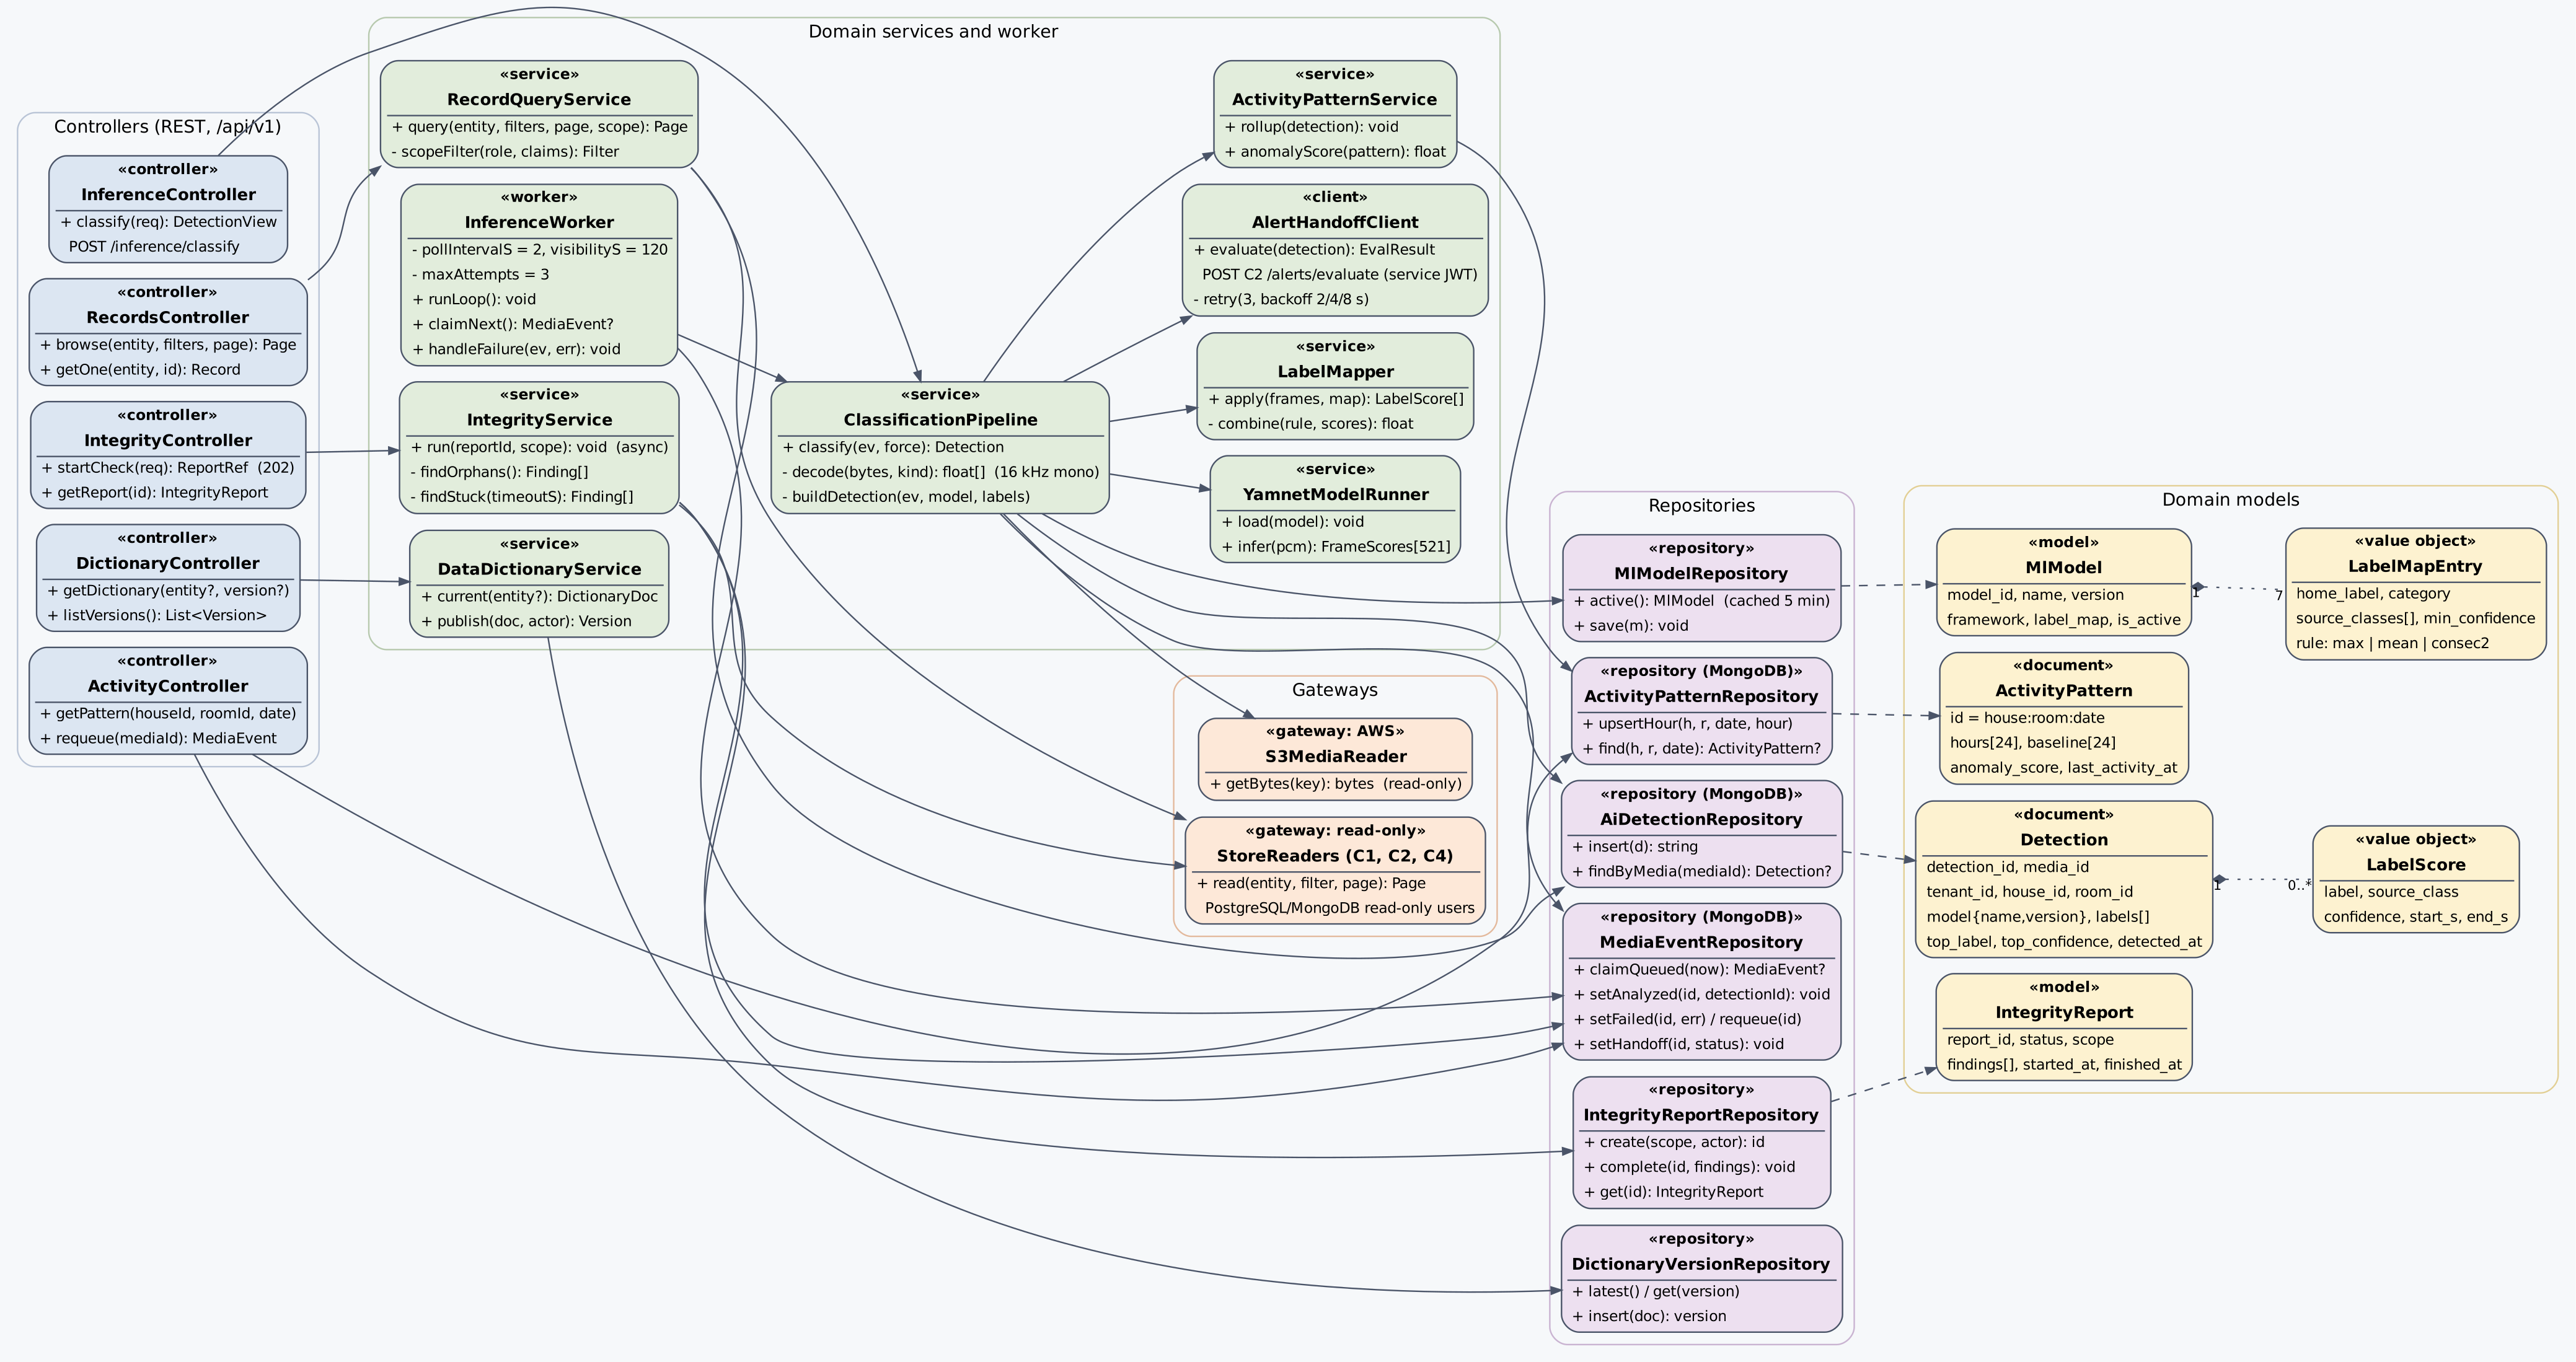
\includegraphics[width=\linewidth,height=0.86\textheight,keepaspectratio]{figures/C3/c3-class}
\captionof{figure}{C3 internal class diagram: controllers, worker and services, repositories, gateways and domain models}\label{fig:c3-class}
\end{landscape}

\begin{longtable}{L{3.6cm}L{1.9cm}L{5.8cm}L{3.5cm}}
\caption{C3 class specification}\label{tab:c3-classspec}\\
\toprule
\textbf{Class} & \textbf{Type} & \textbf{Responsibility} & \textbf{Uses} \\
\midrule
\endfirsthead
\caption[]{C3 class specification (continued)}\\
\toprule
\textbf{Class} & \textbf{Type} & \textbf{Responsibility} & \textbf{Uses} \\
\midrule
\endhead
\texttt{InferenceWorker} & worker & Poll, claim, call pipeline, handle failure and retries & \texttt{MediaEventRepository}, pipeline \\
\texttt{ClassificationPipeline} & service & S3 read, decode, infer, label map, store, rollup, handoff & runner, mapper, repositories, handoff client \\
\texttt{YamnetModelRunner} & service & Load model, infer 521 classes per 0.96 s frame & TensorFlow model file \\
\texttt{LabelMapper} & service & Group classes, threshold, combine frames & \texttt{MlModel.label\_map} \\
\texttt{AlertHandoffClient} & client & POST to C2 with retries & C2 API \\
\texttt{RecordQuery\allowbreak Service} & service & Whitelisted, scoped, paged reads & \texttt{StoreReaders} \\
\texttt{IntegrityService} & service & Async cross-store checks; re-send pending handoffs & readers, report repository \\
\texttt{DataDictionary\allowbreak Service} & service & Serve and publish dictionary versions & \texttt{DictionaryVersion\allowbreak Repository} \\
\texttt{ActivityPattern\allowbreak Service} & service & Hourly counts, baseline, anomaly score & \texttt{ActivityPattern\allowbreak Repository} \\
\bottomrule
\end{longtable}

\subsection{Data and database design}
C3 owns three PostgreSQL tables and two MongoDB collections, and writes only the processing fields of C1's
\texttt{media\_events} (Figure~\ref{fig:c3-er}). Every document carries \texttt{tenant\_id} and \texttt{house\_id} so a
query is scoped the same way as on the relational side.

\figH{C3/c3-er}{0.95}{C3 entity-relationship diagram (white = C3-owned, grey = other components)}{fig:c3-er}

\begin{longtable}{L{4.4cm}L{3.0cm}L{7.2cm}}
\caption{C3 data dictionary (key fields)}\label{tab:c3-dd}\\
\toprule
\textbf{Table / field} & \textbf{Type} & \textbf{Constraint / description} \\
\midrule
\endfirsthead
\caption[]{C3 data dictionary (key fields) (continued)}\\
\toprule
\textbf{Table / field} & \textbf{Type} & \textbf{Constraint / description} \\
\midrule
\endhead
\texttt{ml\_models.label\_map} & JSONB & The label map (Section~\ref{sec:c3-tbd1}); exactly one row \texttt{is\_active} (partial unique index) \\
\texttt{integrity\_reports.status} & VARCHAR CHECK & \texttt{running}, \texttt{done}, \texttt{failed}; \texttt{findings} JSONB \\
\texttt{data\_dictionary\_versions.document} & JSONB & Entities, fields, types, owner component; immutable per version \\
\texttt{ai\_detections.\_id} & UUID string & \texttt{detection\_id}; C2 stores it in \texttt{alerts.detection\_id} \\
\texttt{ai\_detections.media\_id} & UUID string & UNIQUE; link to \texttt{media\_events.\_id} \\
\texttt{ai\_detections.labels[]} & array & \texttt{\{label, confidence, source\_class, start\_s, end\_s\}}, sorted by confidence \\
\texttt{ai\_detections.room\_id} & UUID & Copied from the clip so C2 can match room rules \\
\texttt{activity\_patterns.\_id} & string & \texttt{house:room:date}; \texttt{hours[24]}, \texttt{baseline[24]}, \texttt{anomaly\_score} 0--1 \\
\texttt{media\_events} (C3 fields) & mixed & \texttt{status}, \texttt{attempts}, \texttt{claimed\_at}, \texttt{error}, \texttt{detection\_id}, \texttt{handoff\_status} (\texttt{done}, \texttt{pending}) \\
\bottomrule
\end{longtable}
\textbf{Indexes.} \texttt{ai\_detections \{media\_id:1\}} unique; \texttt{\{house\_id:1, top\_label:1, detected\_at:-1\}};
\texttt{activity\_patterns \{house\_id:1, room\_id:1, date:-1\}}; \texttt{media\_events \{status:1, uploaded\_at:1\}} (claim order, owned by C1).

\subsection{Program function descriptions}
\begin{longtable}{L{4.0cm}L{4.0cm}L{6.6cm}}
\caption{C3 key internal functions}\label{tab:c3-fn}\\
\toprule
\textbf{Function} & \textbf{Inputs $\rightarrow$ outputs} & \textbf{Logic} \\
\midrule
\endfirsthead
\caption[]{C3 key internal functions (continued)}\\
\toprule
\textbf{Function} & \textbf{Inputs $\rightarrow$ outputs} & \textbf{Logic} \\
\midrule
\endhead
\texttt{claimNext()} & none $\rightarrow$ MediaEvent? & Oldest \texttt{queued}, or \texttt{processing} older than 120 s, $\rightarrow$ \texttt{processing}, attempts + 1 \\
\texttt{classify(ev, force)} & clip $\rightarrow$ Detection & S3, decode, YAMNet, label map, store, rollup, handoff \\
\texttt{LabelMapper.\allowbreak apply} & frame scores $\rightarrow$ labels & Per-label threshold and frame-combine rule \\
\texttt{handleFailure(ev, err)} & clip, error $\rightarrow$ void & attempts $<$ 3: \texttt{queued}; else \texttt{failed} \\
\texttt{anomalyScore(p)} & pattern $\rightarrow$ 0--1 & Mean over hours of $\min(1, |c_h-\mu_h|/(3\sigma_h+1))$ vs 28-day baseline \\
\texttt{scopeFilter(role, claims)} & claims $\rightarrow$ filter & Table~\ref{tab:c3-scope-dt} \\
\bottomrule
\end{longtable}

\figH{C3/c3-inference-flow}{0.55}{Inference worker flowchart: claim, decode, infer, map labels, store, hand off to C2, with retry and failure paths}{fig:c3-inference}

\begin{Shaded}
\begin{Code}
function classify(ev, force=false):
    if aiDetections.findByMedia(ev._id) and not force: raise 409 already_analyzed
    pcm    = decodeTo16kMono(s3.getBytes(ev.s3.key), ev.media_kind)   # video -> audio track
    model  = mlModels.active()                                        # cached; carries label_map
    labels = labelMapper.apply(yamnet.infer(pcm), model.label_map)   # may be empty
    det = Detection(id=uuid4(), media_id=ev._id, tenant_id=ev.tenant_id, house_id=ev.house_id,
                    room_id=ev.room_id, model=(model.name, model.version), labels=labels,
                    top_label=labels[0].label if labels else "none",
                    top_confidence=labels[0].confidence if labels else 0.0, detected_at=now())
    aiDetections.upsertByMedia(det)
    mediaEvents.setAnalyzed(ev._id, det.id)
    activity.rollup(det)
    try:    handoff.evaluate(det); mediaEvents.setHandoff(ev._id, "done")     # 3 retries inside
    except: mediaEvents.setHandoff(ev._id, "pending")                         # re-sent by integrity job
    return det

function apply(frames, label_map):                    # frames: n x 521 scores
    out = []
    for e in label_map.entries:                        # one entry per home label
        perFrame = [max(f[c] for c in e.source_classes) for f in frames]
        s = max(perFrame) if e.rule == "max" else mean(perFrame) if e.rule == "mean" \
            else max(min(perFrame[i], perFrame[i+1]) for i in range(len(perFrame)-1))   # consec2
        if s >= e.min_confidence: out.append(LabelScore(e.home_label, s))
    return sorted(out, by=confidence, desc=True)
\end{Code}
\end{Shaded}

\subsection{Behavior: clip state machine}
Figure~\ref{fig:c3-state} is the clip state machine as C3 drives it. The claim makes \texttt{queued} to
\texttt{processing} atomic; an error or a 120 s visibility timeout returns the clip to \texttt{queued} while
attempts $<$ 3; the third failure sets \texttt{failed}, from which an operator can requeue.

\figH{C3/c3-mediaevent-state}{1.0}{Clip state machine in media\_events: queued, processing, analyzed, failed}{fig:c3-state}

\subsection{Behavior: sequence diagrams}\label{sec:c3-seq}
Figure~\ref{fig:c3-seq} is Classify a clip (UC-03) on the worker path, ending with the handoff to C2 and its
retry branch. The on-demand \texttt{POST /inference/classify} runs the same pipeline without the claim.
Figure~\ref{fig:c3-seq-records} shows cloud staff browsing scoped records and running an asynchronous integrity check.

\figH{C3/c3-seq-classify}{1.0}{Sequence (a): worker claims, classifies, stores and hands off to C2 (UC-03)}{fig:c3-seq}
\figH{C3/c3-seq-records}{0.95}{Sequence (b): scoped record browsing and an asynchronous integrity check}{fig:c3-seq-records}

% ============================================================================
\section{Component Business Logic}

\subsection{The label map (TBD-1, resolved)}\label{sec:c3-tbd1}
This resolves TBD-1: the 521 YAMNet AudioSet classes map to seven home labels. YAMNet scores a clip in about
0.96-second frames, so a 10-second clip gives about ten frames. Thresholds are design defaults to be validated in
D3 (TBD-3). A fall is inferred from its sound through \texttt{fall\_indicator}. C2's alert types use these labels as triggers.

\begin{longtable}{L{2.6cm}L{1.9cm}L{5.0cm}L{1.6cm}L{2.4cm}}
\caption{Label map}\\
\toprule
\textbf{Home label} & \textbf{Category} & \textbf{YAMNet source classes (examples)} & \textbf{Min conf.} & \textbf{Frame rule} \\
\midrule
\endfirsthead
\caption[]{Label map (continued)}\\
\toprule
\textbf{Home label} & \textbf{Category} & \textbf{YAMNet source classes (examples)} & \textbf{Min conf.} & \textbf{Frame rule} \\
\midrule
\endhead
\texttt{smoke\_alarm} & emergency & Smoke detector, smoke alarm; Fire alarm; Alarm & 0.50 & max \\
\texttt{distress\_sound} & emergency & Screaming; Shout; Yell; Crying, sobbing & 0.60 & 2 consecutive \\
\texttt{glass\_break} & security & Glass; Shatter; Breaking & 0.55 & max \\
\texttt{fall\_indicator} & safety & Thump, thud; Bang; Slam & 0.65 & 2 consecutive \\
\texttt{cough} & wellness & Cough; Throat clearing & 0.55 & mean \\
\texttt{speech} & wellness & Speech; Conversation & 0.50 & mean \\
\texttt{dog} & wellness & Dog; Bark & 0.55 & max \\
\bottomrule
\end{longtable}

\subsection{Frame-combine selection}
\begin{longtable}{L{5.0cm}L{3.6cm}L{5.4cm}}
\caption{Frame-combine rule by event character}\\
\toprule
\textbf{Event character} & \textbf{Rule} & \textbf{Why} \\
\midrule
\endfirsthead
\caption[]{Frame-combine rule by event character (continued)}\\
\toprule
\textbf{Event character} & \textbf{Rule} & \textbf{Why} \\
\midrule
\endhead
Sharp, short, loud (alarm, glass, bark) & max over frames & One strong frame is the event \\
Sustained but startle-prone (scream, thud) & 2 consecutive frames & Rejects a single spurious frame \\
Diffuse, ongoing (speech, cough) & mean over frames & Rewards presence across the clip \\
\bottomrule
\end{longtable}

\subsection{Worker claim and retry}
\begin{longtable}{L{3.4cm}L{3.0cm}L{8.2cm}}
\caption{Claim and retry}\\
\toprule
\textbf{Status} & \textbf{Condition} & \textbf{Action} \\
\midrule
\endfirsthead
\caption[]{Claim and retry (continued)}\\
\toprule
\textbf{Status} & \textbf{Condition} & \textbf{Action} \\
\midrule
\endhead
\texttt{queued} & oldest first & Claim: \texttt{processing}, attempts + 1 \\
\texttt{processing} & error, attempts $<$ 3 & Back to \texttt{queued} \\
\texttt{processing} & older than 120 s & Reclaimable (worker crashed) \\
\texttt{processing} & error, attempts = 3 & \texttt{failed}, error logged \\
\texttt{failed} & operator requeue & \texttt{queued}, attempts = 0 \\
\bottomrule
\end{longtable}

\subsection{Record scope decision table}
\begin{longtable}{L{3.6cm}L{3.6cm}L{3.6cm}L{3.8cm}}
\caption{Record browsing scope}\label{tab:c3-scope-dt}\\
\toprule
\textbf{Entity} & \textbf{house\_owner} & \textbf{iot\_staff} & \textbf{cloud\_staff} \\
\midrule
\endfirsthead
\caption[]{Record browsing scope (continued)}\\
\toprule
\textbf{Entity} & \textbf{house\_owner} & \textbf{iot\_staff} & \textbf{cloud\_staff} \\
\midrule
\endhead
houses, rooms, feeds, clips & own \texttt{house\_ids} & own tenant & any tenant \\
detections, activity\_patterns & own \texttt{house\_ids} & own tenant & any tenant \\
alerts & own \texttt{house\_ids} & no (403) & any tenant \\
dictionary, integrity, requeue & no & no & yes \\
\bottomrule
\end{longtable}

\subsection{Integrity validation}
\begin{longtable}{L{4.2cm}L{5.2cm}L{5.2cm}}
\caption{Integrity checks}\\
\toprule
\textbf{Condition} & \textbf{Check} & \textbf{Reported action} \\
\midrule
\endfirsthead
\caption[]{Integrity checks (continued)}\\
\toprule
\textbf{Condition} & \textbf{Check} & \textbf{Reported action} \\
\midrule
\endhead
Detection with no clip & \texttt{ai\_detections.media\_id} not in \texttt{media\_events} & Orphan detection (high) \\
Clip analysed, no detection & \texttt{status = analyzed}, no \texttt{detection\_id} & Missing detection; re-classify (medium) \\
Alert with dangling link & \texttt{alerts.detection\_id} not in \texttt{ai\_detections} & Broken cross-store link (high) \\
Clip stuck processing & \texttt{processing} older than 120 s & Requeue candidate (medium) \\
Handoff pending & \texttt{handoff\_status = pending} & Re-send to C2 automatically (low) \\
\bottomrule
\end{longtable}

\subsection{Anomaly score banding}
\begin{longtable}{L{3.6cm}L{4.0cm}L{6.8cm}}
\caption{Anomaly score interpretation}\\
\toprule
\textbf{Score} & \textbf{Band} & \textbf{Shown as} \\
\midrule
\endfirsthead
\caption[]{Anomaly score interpretation (continued)}\\
\toprule
\textbf{Score} & \textbf{Band} & \textbf{Shown as} \\
\midrule
\endhead
$<$ 0.30 & normal & No marker \\
0.30 -- 0.60 & unusual & ``Unusual activity'' note on Home Overview \\
$\geq$ 0.60 & anomalous & Highlighted room card; listed for staff review \\
\bottomrule
\end{longtable}

% ============================================================================
\section{Component Graphic User Interface Design}

\subsection{GUI style}
\begin{longtable}{L{3.0cm}L{11.8cm}}
\caption{C3 GUI style}\\
\toprule
\textbf{Element} & \textbf{Rule} \\
\midrule
\endfirsthead
\caption[]{C3 GUI style (continued)}\\
\toprule
\textbf{Element} & \textbf{Rule} \\
\midrule
\endhead
Workspace & One page family in the cloud-staff workspace (\texttt{/ops/records}, \texttt{/ops/dictionary}, \texttt{/ops/integrity}) inside C4's shell. \\
Data views & Entity chips, filter bar and paged table; IDs shortened with copy-on-click; times in the viewer's zone with UTC on hover. \\
Status encoding & Clip status and finding severity as icon + word, never colour alone. \\
Long tasks & Integrity check shows a running state and polls the report every 5 s. \\
Safety & Only read and requeue actions; no edit or delete of records from the UI. \\
\bottomrule
\end{longtable}

\subsection{Storyboard}
Figure~\ref{fig:c3-story}: path~A shows a clip being queued, claimed, classified and handed off (1--4). Path~B shows
cloud staff browsing detections, paging scoped results, running an integrity check and acting on its findings (5--8).

\figH{C3/c3-storyboard}{1.0}{C3 storyboard: automatic classification and staff data checks}{fig:c3-story}

\subsection{Function partition tree}
\figH{C3/c3-gui-tree}{0.66}{C3 GUI function partition: Database Records and its functions}{fig:c3-gui-tree}

\subsection{UI markup diagram and wireframe}
\figH{C3/c3-wireframe-records}{0.9}{UI markup of Database Records: entity chips, filters, scoped table, integrity panel and actions}{fig:c3-wireframe}

\begin{longtable}{L{0.6cm}L{3.0cm}L{2.6cm}L{4.0cm}L{4.4cm}}
\caption{Database Records markup legend}\label{tab:c3-markup}\\
\toprule
\textbf{\#} & \textbf{Element} & \textbf{Template} & \textbf{Data source} & \textbf{Behaviour} \\
\midrule
\endfirsthead
\caption[]{Database Records markup legend (continued)}\\
\toprule
\textbf{\#} & \textbf{Element} & \textbf{Template} & \textbf{Data source} & \textbf{Behaviour} \\
\midrule
\endhead
1 & Navigation & AppShell (C4) & JWT role & Ops links only for cloud staff \\
2 & Entity chips & ChipGroup & entity whitelist & Selecting reloads the table \\
3 & Filter bar & FilterBar & houses in scope & House, date range, field filter \\
4 & Results table & DataTable & \texttt{GET /records/\{entity\}} & Paged 25 rows; shows scope \\
5 & Integrity panel & FindingList & \texttt{GET /integrity-reports/\{id\}} & Severity icon + word \\
6 & Actions & ActionBar & \texttt{POST /integrity-checks}, dictionary, requeue & Run (202), export, requeue failed clips \\
\bottomrule
\end{longtable}

\subsection{GUI templates}
\begin{longtable}{L{3.0cm}L{4.2cm}L{7.6cm}}
\caption{GUI templates used by C3}\\
\toprule
\textbf{Template} & \textbf{Used on} & \textbf{Props / behaviour} \\
\midrule
\endfirsthead
\caption[]{GUI templates used by C3 (continued)}\\
\toprule
\textbf{Template} & \textbf{Used on} & \textbf{Props / behaviour} \\
\midrule
\endhead
DataTable & Records, dictionary & Server-side paging and sort \\
FilterBar & Records & House picker, date range, field filter \\
ChipGroup & Records & Single-select entity \\
FindingList & Integrity & Findings with severity, link to the record \\
StatusChip & Records & Clip status icon + word \\
\bottomrule
\end{longtable}
